\documentclass[a4paper]{article}
\usepackage[dutch]{babel}
\usepackage[utf8x]{inputenc}
\usepackage{siunitx,amsmath, epic, eepic, float, subfig, amsfonts, color, amsthm, textcomp, microtype, fullpage}
\usepackage[parfill]{parskip}
\usepackage[pdftex]{graphicx}
\usepackage{color}
\definecolor{bluekeywords}{rgb}{0.13,0.13,1}
\definecolor{greencomments}{rgb}{0,0.5,0}
\definecolor{redstrings}{rgb}{0.9,0,0}
\usepackage[font=small,format=plain,labelfont=bf,textfont=it]{caption}
\usepackage[linkcolor=black,urlcolor=blue,citecolor=black]{hyperref}
\hypersetup{colorlinks=true}
\newcommand{\HRule}{\rule{\linewidth}{0.5mm}}
\linespread{1.3}
\usepackage[final]{pdfpages}
\usepackage[T1]{fontenc}
\usepackage{lmodern}
\usepackage{beramono}
\usepackage{helvet}
\renewcommand*{\familydefault}{\sfdefault}

\begin{document}
\begin{titlepage}
\begin{center}

\includegraphics[width=0.5\textwidth]{src/logo.pdf}~\\[1cm]


\textsc{\Large Beroepsethiek}\\[0.5cm]

\HRule \\[0.4cm]
{ \LARGE \bfseries Vergelijking van de situatie in Irak en Syrië met het conflict in Joegoslavië }\\[0.4cm]
{\large \textit{Wat ging er fout en hoe vermijden we het?}}\\[0.2cm]

\HRule \\[1.5cm]

\begin{minipage}{0.4\textwidth}
\begin{flushleft} \large
\emph{Door:}\\
Haroen \textsc{Viaene}\\

\end{flushleft}
\end{minipage}
\begin{minipage}{0.4\textwidth}
\begin{flushright} \large
\large{3$^{\text{de}}$ fase bachelor Elektronica-ICT}\\
\end{flushright}
\end{minipage}

\vfill

{\large 2016-2017}

\end{center}
\end{titlepage}

\newpage

\begin{abstract}
\noindent Humanitaire acties moeten op een andere manier gebeuren dan die nu gebeuren, door op een burgerlijkere manier om te gaan met conflicten kunnen we de fouten van vroeger tegengaan.
\end{abstract}

\section{Aanloop} % (fold)
\label{sec:aanloop}

In het Midden-Oosten en in de Balkan liep de geschiedenis op een vergelijkbare manier. Ongeveer honderd jaar geleden waren die beide deel van grote rijken die aan het vervallen waren, waarna Europese kolonisatie grenzen maakte die weinig rekening hielden met etnische grenzen.

Hierdoor ontstonden er op vergelijkbare wijze spanningen die op het moment dat er ``zwakkere leiders'' aan het hoofd van die naties stonden ontploften.

Hierdoor was er een klimaat die het vormen van (volgens sommigen terroristische, volgens andere nationalistische, en volgens nog andere volks-) groeperingen die onder het mom van religieuze en andere doelen mogelijk maakt.

% section aanloop (end)

\section{Genomen acties} % (fold)

\label{sec:genomen_acties}
Initieel deden Westerse landen heel weinig, zowel in het Midden-Oosten als in de Balkan-conflicten. Het is makkelijk te zeggen dat hier samenzweringen en opportunisme achter zitten, maar daar zal ik nu niet over oordelen.

Daarna werd er in Joegoslavië -- tegen de aanbeveling van de UN -- een grond- en luchtoffensief ingezet. Deze had als voornamelijk doel om de oorlogsmisdaden die Milosevic e.d. pleegden te stoppen, maar op die manier steunde het ook de separatistische Kosovaarse bewegingen.

In Syrië werd er in tegenstelling tot andere Midden-Oosterse gebieden initieel geen actie genomen; in Irak en Afghanistan wel. Pas op het moment dat er verplicht aandacht komt aan het probleem door o.a. aanslagen in Europa werd er actie ondernomen. Ditmaal gaat het eerder om aanwezigheid en gerichte bombardementen\footnote{uiteraard is dit moeilijk te zeggen vanuit onze bronnen}, maar hoe weten we hoe ernstig die zijn? We hadden hetzelfde gevoel zeventien jaar geleden, maar achteraf bleek dat er verschillende serieus foute dingen gebeurd zijn door NAVO-militairen.

% section genomen_acties (end)

\section{Mogelijke acties} % (fold)
\label{sec:mogelijke_acties}

Er zijn heel veel mogelijke manieren om een oplossing te vinden voor situaties waarmee je het politiek niet eens bent. Hier zal ik focussen op de humanitaire aspecten, waardoor het mogelijk is dat deze oplossingen bepaalde dingen over het hoofd zien vanuit bijvoorbeeld economisch standpunt.

Er zijn duidelijke voordelen te bedenken bij een harde militaire aanval. Net zoals eerder in de geschiedenis bewezen, kan een harde aanval met veel burgerlijke, infrastructurele, historische en andere schade wel een positief effect hebben. Zo stopt het meestal verdere escalatie en het langer uitlopen van het conflict. Jammer genoeg is het moeilijk zeker te zijn van dat effect, omdat het op verschillende vlakken goed uitkomt om een aanhoudend effect te behouden. Zo zitten veel van de militaire \emph{contractors} ook in de heropbouw-business.

Verder is het ook heel belangrijk dat er \emph{iets} gebeurt. Zoals we eerder al zagen heeft het weinig voordeel om daden die tegen essentiële rechten ingaan door de vingers te zien. In Irak hebben de Verenigde Staten beslist om hun invloeden in de oliesector in een hoog vaandel te houden, en er voor te zorgen dat er productie kon blijven -- een gelijkaardig verhaal in Libië. Om een ``duidelijk signaal'' te geven werd er heel hard militair ingezet, met als gevolg dat er een politieke spanning ontstaat die uitmondt in steun voor fractiegroeperingen.

Het is dus duidelijk dat militair ingrijpen -- naast de positieve gevolgen -- niet de juiste oplossing is. Een andere oplossing (die aangerijkt wordt in \emph{Yugoslavia, Syria and Iraq - lessons learnable?} \cite{transconflict}) is om niet per se de foute leiders (Milosevic, Saddam, Assad, Gaddafi \dots) zo snel mogelijk af te zetten, maar ermee samenwerken en echte democratische verkiezingen op te stellen.

Jammer genoeg speelt bij verkiezingen populisme een heel grote rol -- bij ons ook, niet enkel bij landen waar het fenomeen recent is. Nationalisme is een gevoel dat zeer aantrekkelijk is wanneer landen in slechtere staat zijn. Dat zien we op allerlei verschillende momenten, ook zo met recente verkiezingen in het Westen, waardoor het aanmoedigen van verkiezingen wanneer de staat van het land slecht is tot extreme regeringen kan leiden.

\begin{quote}
  ``if you want to maintain the stability of internally divided states (especially in rough neighborhoods), it might be better to work with the leaders you have'' \cite{transconflict}
\end{quote}

Hoe onlogisch het in eerste opzicht lijkt, toch is het dus beter samen te werken dan tegen te werken. Een land destabiliseren is niet de manier om het terug in orde te krijgen.

\begin{quote}
  ``collective identity remains the essential basis for political power as wielded by those seeking to gain and hold it and as recognized by those ready to follow.'' \cite{transconflict}
\end{quote}

Wanneer de collectieve identiteit van een land wegvalt (de naam, een sterke leider, de grenzen) wordt er vanuit menselijke natuur terug gevallen op andere dingen die groepen maken. Dat is bijvoorbeeld religie, waarden, regio's \dots In landen met veel verschillende etniciteiten kan dit aflopen in burgeroorlogen en afrekeningen. Daarom is het best om de noden te zien van alle groepen, en:

\begin{quote}
  ``the process of breakup once underway is essentially unstoppable.'' \cite{transconflict}
\end{quote}

Eens bepaalde stappen gezet zijn naar onafhankelijkheid van een regio is het niet slim die op allerlei manieren tegen te gaan. Natuurlijk is dat een heel moeilijk probleem, want wat doe je als die ``staat'' die erkenning wil een overduidelijk repressief regime is? Wat als je ziet dat die staat essentiële rechten van de mens niet respecteert?

Zoals in \emph{Het verdriet van Syrië} \cite{verdriet} te lezen ziet het er naar uit dat Assad terug veel macht zal krijgen in de komende periode. Is dit het moment waarop we diplomatisch en op andere niet-militaire manieren omgaan met een Syrië onder Assad? Kunnen we überhaupt wel nog beslissingen maken met Trump als president van de VS en dus met vetorecht over de NAVO?

Moeten we IS aanvaarden als land en op een diplomatische manier dingen proberen oplossen? Is dat wel mogelijk? Moeten we troepen sturen om op te bouwen als we weten dat het snel vernietigd zal worden? Op welke manier moeten we ons in een conflict ``moeien'' dat het onze niet is? Maken we deel uit van het conflict?

Dit is zo'n ingewikkeld onderwerp dat ik daar zomaar geen antwoorden op kan geven, maar ik ben toch van mening dat zwaar militair actie ondernemen niet alleen humanitair, niet alleen vanuit cultureel maar ook uit langetermijnsperspectief geen goed idee is.

% section mogelijke_acties (end)

\section{Bedenkingen} % (fold)
\label{sec:bedenkingen}

Het is te merken dat bij onderwerpen zoals deze, je heel gekleurd nieuws krijgt afhankelijk waar je je nieuws haalt. Niets is echt onafhankelijk omdat verschillende bronnen aangesproken worden afhankelijk van welke persoon het schrijft, en welke ``kant van de geschiedenis'' je aan staat.

Zo is \emph{Kosovo independence: Dilemmas on the NATO’s aggression in 1999} \cite{kosovo} duidelijk geschreven vanuit een Servisch standpunt, en \emph{Yugoslavia, Syria and Iraq - lessons learnable?} \cite{transconflict} vanuit een Amerikaans. Ik heb hier bewust voor gekozen omdat ik vind dat het altijd interessant is om situaties te bekijken van de ``andere kant''.

Verder merk ik ook dat ik graag meer achtergrond zou hebben voordien me uit te spreken over deze onderwerpen; ik merk zeer duidelijk dat ik niet weet wat ik kan geloven en wat niet, nummers verschillen heel significant van de ene bron tot de andere wat conclusies maken bemoeilijkt.

% section bedenkingen (end)

\begin{raggedright}
  \begin{thebibliography}{9}

  \bibitem{transconflict}
    \textbf{Yugoslavia, Syria and Iraq - lessons learnable?}
    Gerard Gallucci,
    TransConflict
    [Opgehaald 25 november 2016]
    \url{http://www.transconflict.com/2015/06/yugoslavia-syria-and-iraq-lessons-learnable-096/}

  \bibitem{toolkit}
    \textbf{Syrian army troops advance on Aleppo as Nato calls air strikes `blatant violation of international law'}
    Bethan McKernan,
    The Independent
    [opgehaald 26 november 2016]
    \url{http://www.independent.co.uk/news/syria-war-aleppo-attack-assad-army-ground-troops-in-city-nato-air-strikes-a7332591.html}

  \bibitem{kosovo}
    \textbf{Kosovo independence: Dilemmas on the NATO’s aggression in 1999}
    Prof. Dr. Vladislav B. Sotirovic,
    Modern Democracy
    [Opgehaald 20 november 2016]
    \url{http://moderndiplomacy.eu/index.php?option=com_k2&view=item&id=1390:kosovo-independence-dilemmas-on-the-nato-s-aggression-in-1999&Itemid=569}

  \bibitem{verdriet}
    \textbf{Het verdriet van Syrië}
    Chams Eddine Zaougui,
    De Standaard
    [opgehaald 28 november 2016]
    \url{http://www.standaard.be/cnt/dmf20161127_02594608}
  \end{thebibliography}
\end{raggedright}

\section{Bijlagen} % (fold)
\label{sec:bijlagen}

In bijlage drie van de artikels waaruit ik informatie haalde

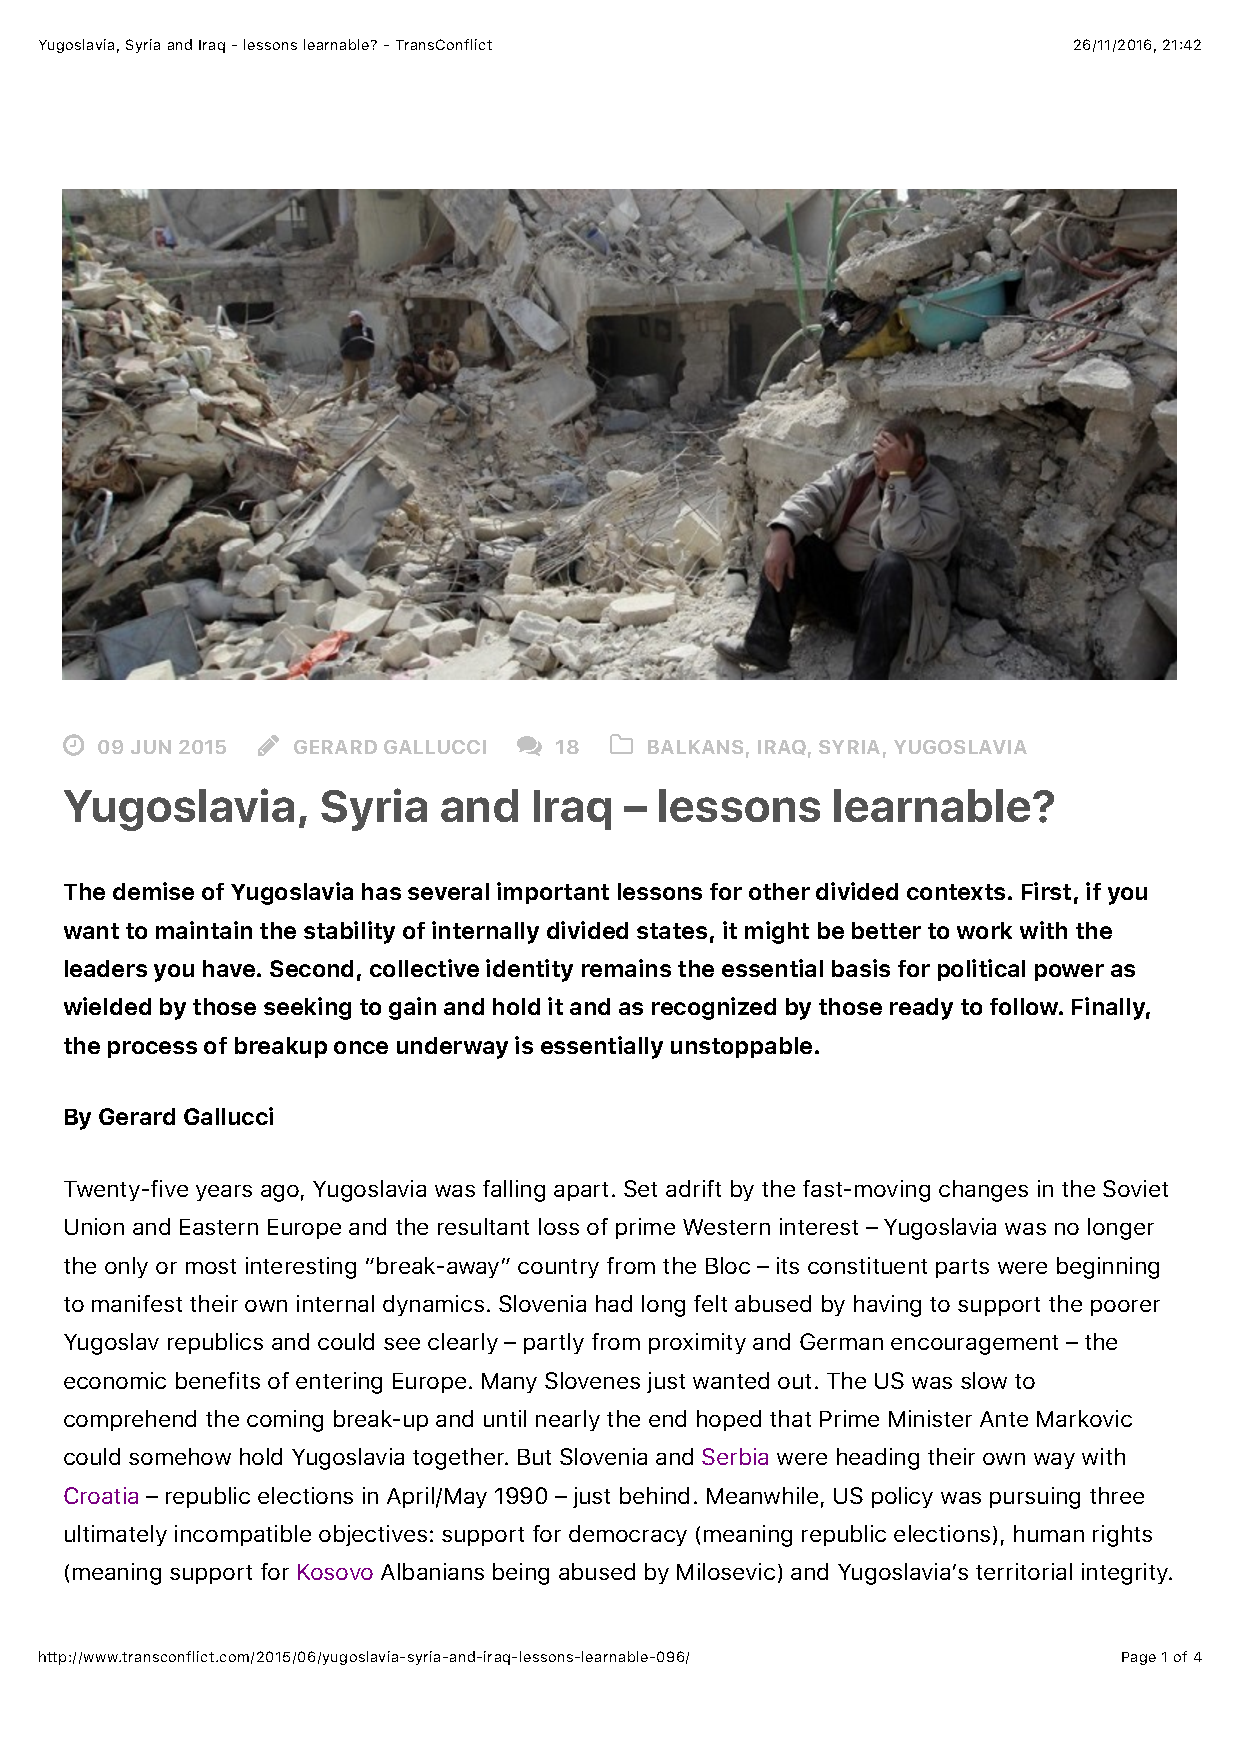
\includepdf[pages=-]{src/lessons.pdf}
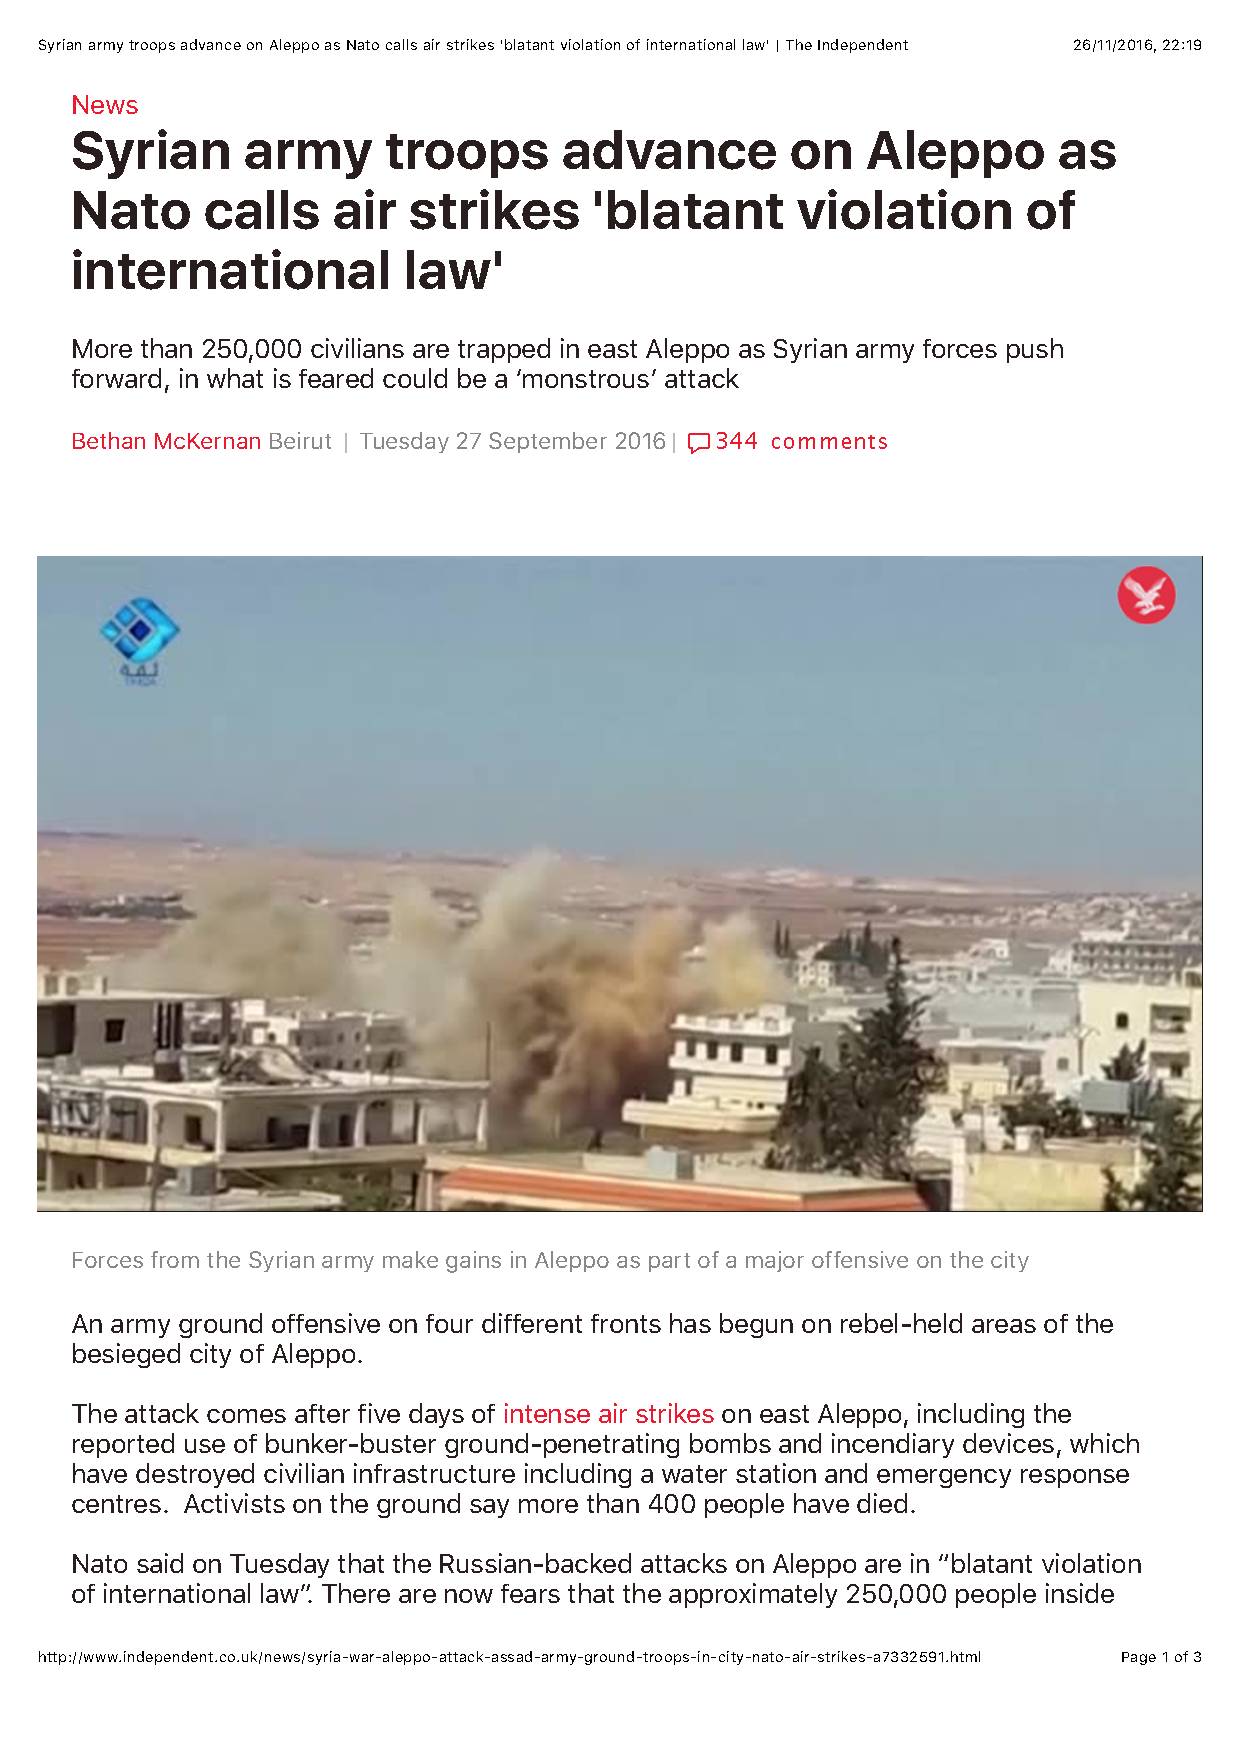
\includepdf[pages=-]{src/syria.pdf}
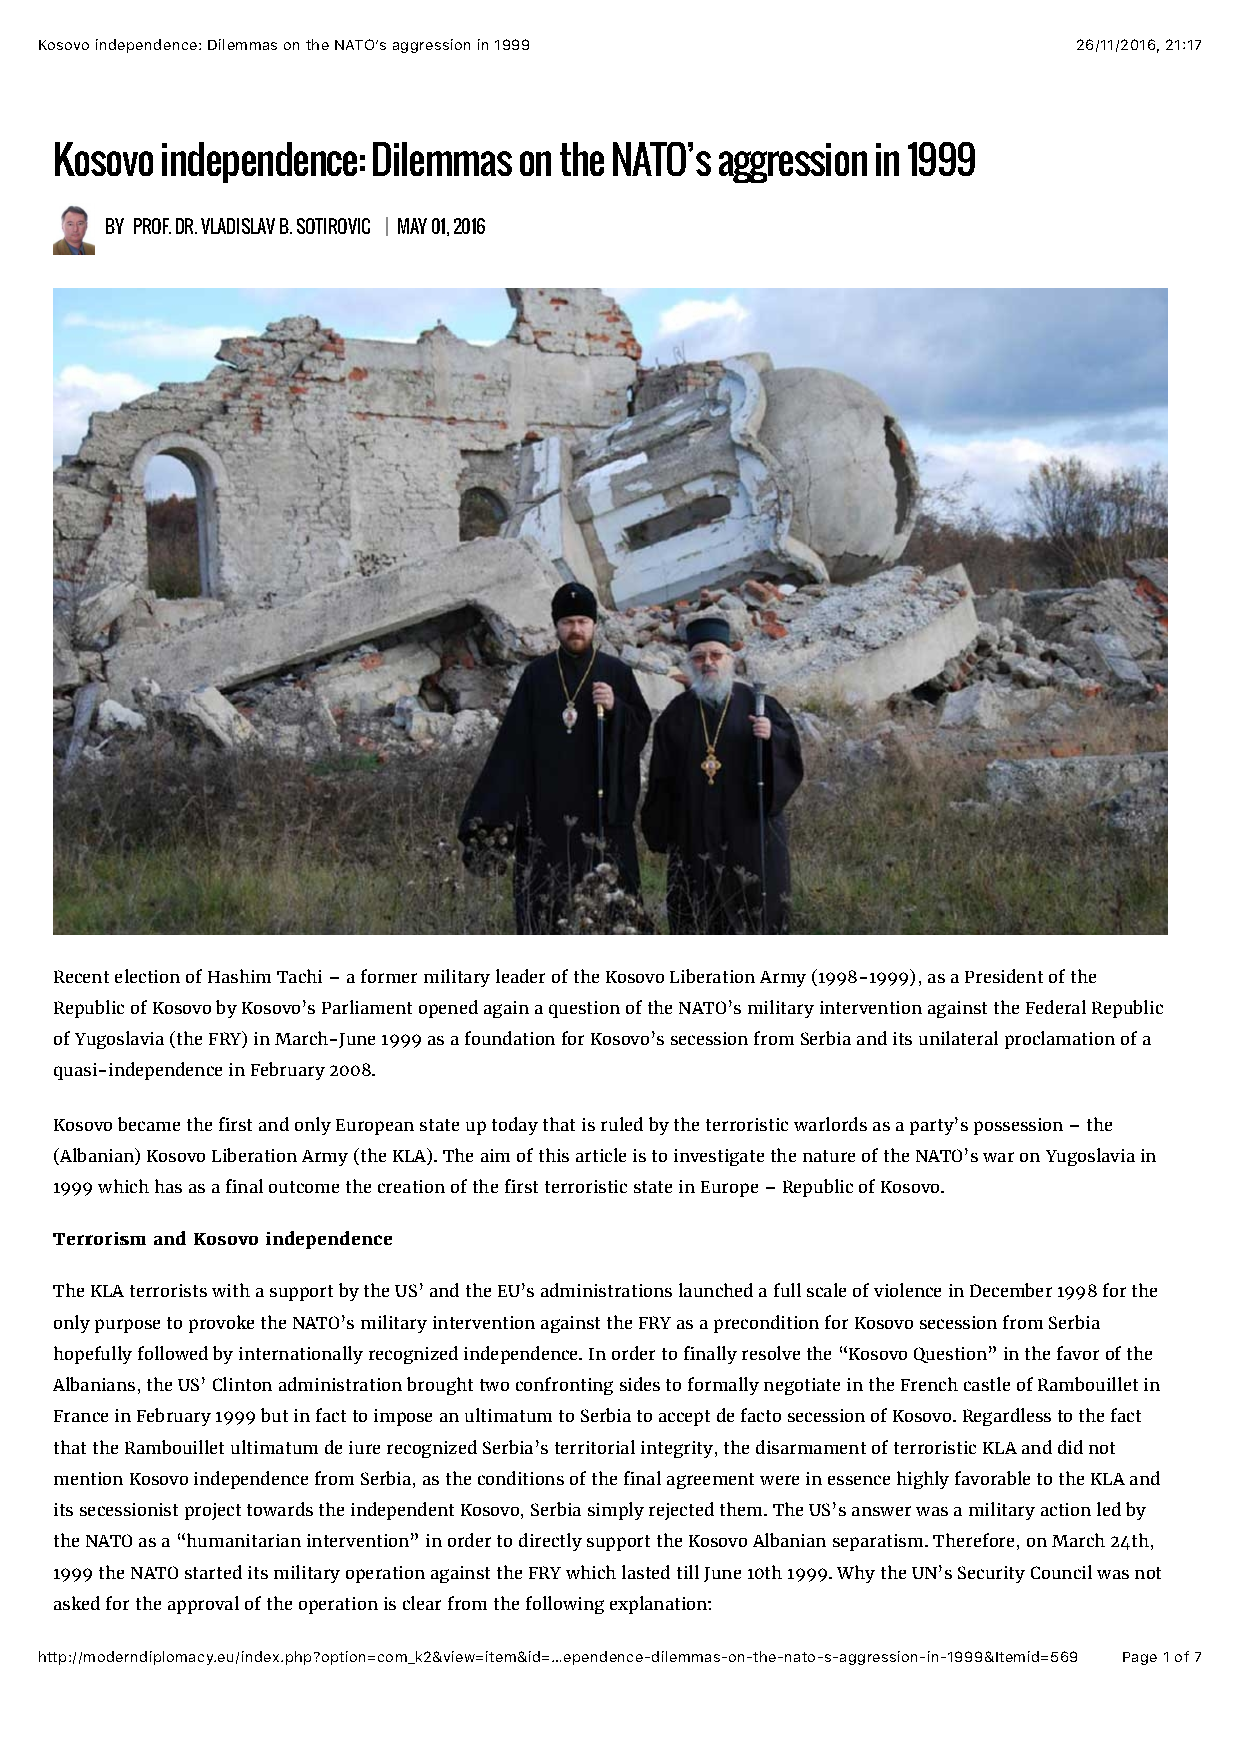
\includepdf[pages=-]{src/kosovo.pdf}
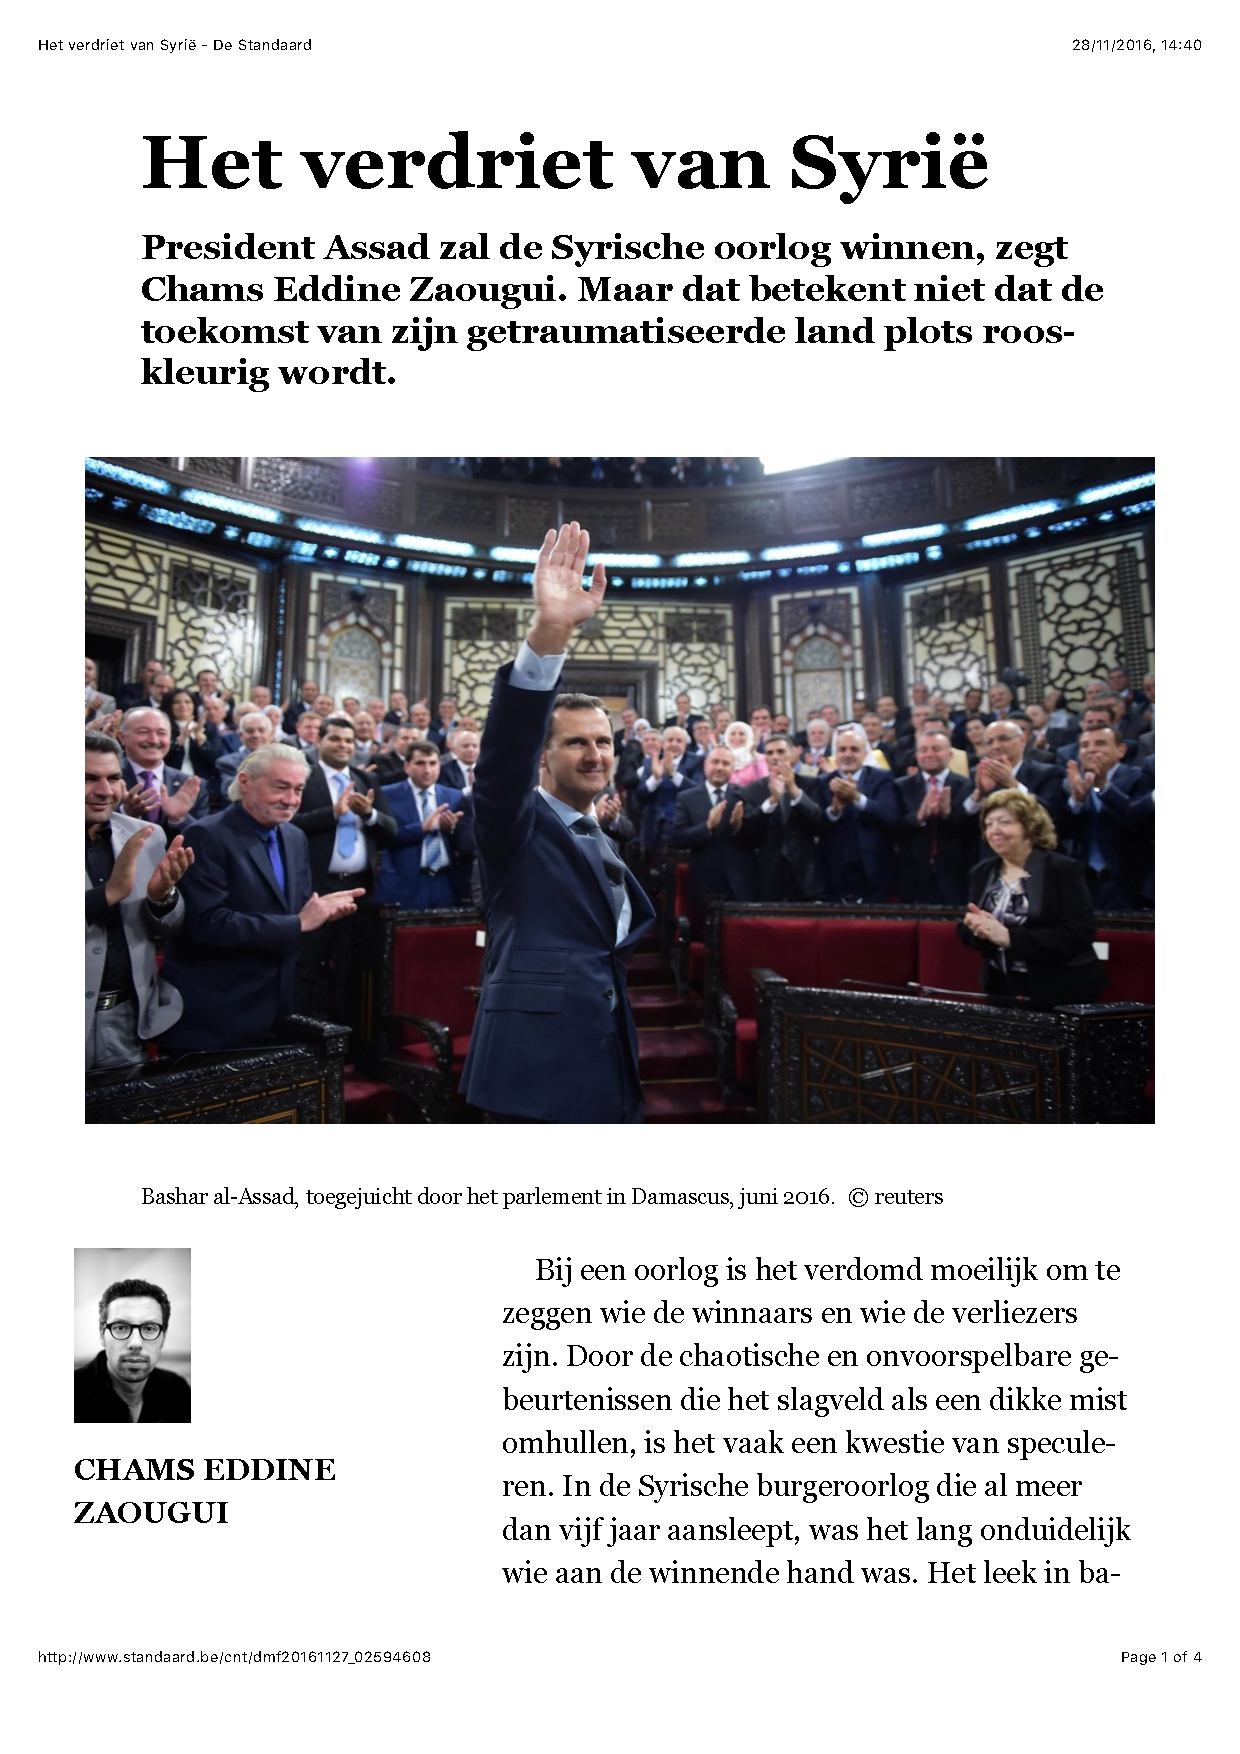
\includepdf[pages=-]{src/verdriet.pdf}

% section bijlagen (end)

\end{document}
